\documentclass[12pt,fleqn]{article}\usepackage{../common}
\begin{document}
Boltzman Makinalari (Rasgele Hopfield Aglari) 

Alttaki ifade bir Boltmann dagilimini gosterir, 

$$  
\mlabel{3}
P(x;W) = \frac{1}{Z(W)} 
\exp \bigg[ \frac{1}{2} x^T W x \bigg]
$$

ki $x$ cok boyutlu ve -1,+1 degerleri iceren bir vektor, $W$ simetrik ve
caprazinda (diagonal) sifir iceren bir matristir, $n \times d$
boyutlarindaki bir veri icin $d \times d$ boyutlarinda olacaktir.  Bolzmann
Makinalari (BM), Kisitli Bolzmann Makinalari (Restricted Bolzmann Machines)
kavramina gecis yapmadan once iyi bir durak noktasi. 

BM $W$ icinde aslinda tum degiskenlerin ikisel iliskisini icerir. $W$ cok
degiskenli Gaussian dagilimindaki $\Sigma$'da oldugu gibi ikisel
baglantilari saptar. Veriden $W$'yu ogrenmek icin olurlugu hesaplamak
lazim. Olurluk (likelihood)

$$  
\prod _{n=1}^{N} P(x^{(n)};W) = \frac{1}{Z(W)} 
\exp \bigg[ \frac{1}{2} x^{(n)^T} W x^{(n)} \bigg]
$$

Log olurluk

$$  
\mlabel{1}
\mathcal{L} = \ln \big( \prod _{n=1}^{N} P(x^{(n)};W) \big) = 
\sum _{n=1}^{N} \bigg[ \frac{1}{2} x^{(n)^T} W x^{(n)} - \ln Z(W) \bigg]
$$

Birazdan $\frac{\partial \mathcal L}{\partial w_{ij}}$ turevini alacagiz, o sirada $\ln Z(W)$'nin turevi lazim, 
daha dogrusu $Z(W)$'yi nasil turevi alinir hale getiririz?

$Z(W)$ normalizasyon sabiti olduguna gore, dagilimin geri kalaninin
sonsuzlar uzerinden entegrali (ya da toplami) normalizasyon sabitine
esittir, 

$$ 
Z(W) = \sum_x  \exp \bigg[ \frac{1}{2} x^T W x \bigg]
 $$

$$ 
\ln Z(W) = \ln \bigg[ \sum_x  \exp \big( \frac{1}{2} x^T W x \big) \bigg]
 $$

Log bazli turev alinca log icindeki hersey oldugu gibi bolume gider, ve log
icindekinin turevi alinirak bolume koyulur. Fakat log icine dikkatli
bakarsak bu zaten $Z(W)$'nin tanimidir, boylece denklemi temizleme sansi
dogdu, bolume hemen $Z(W)$ deriz, ve turevi log'un icine uygulariz,


$$ 
\frac{\partial}{\partial w_{ij}} \ln Z(W) = 
\frac{1}{Z(W)}
\bigg[ 
\sum_x \frac{\partial}{\partial w_{ij}} \exp \big( \frac{1}{2} x^T W x \big) 
\bigg]
 $$


$$ 
\mlabel{2}
\frac{\partial}{\partial w_{ij}} \exp \big( \frac{1}{2} x^T W x \big)  = 
\frac{1}{2}  \exp \big( \frac{1}{2} x^T W x \big) 
\frac{\partial}{\partial w_{ij}}x^T W x
$$

(2)'in icindeki bolumu acalim,

$$ \frac{\partial}{\partial w_{ij}}x^T W x = x_i x_j $$

Simdi (2)'ye geri koyalim,

$$ =  \frac{1}{2}  \exp \big( \frac{1}{2} x^T W x \big) x_i x_j$$

$$ 
\frac{\partial}{\partial w_{ij}} \ln Z(W) = 
\frac{1}{Z(W)}
\bigg[ 
\sum_x \frac{1}{2}  \exp \big( \frac{1}{2} x^T W x \big) x_i x_j
\bigg]
$$

$$ 
= 
\frac{1}{2}  \sum_x \frac{1}{Z(W)}  \exp \big( \frac{1}{2} x^T W x \big) x_i x_j
$$

$$ 
= 
\frac{1}{2}  \sum_x P(x;W) x_i x_j
$$

Ustteki son ifadede bir kisaltma kullanalim,

$$ 
\mlabel{4}
\sum_x P(x;W) x_i x_j =  <x_i,x_j>_{P(x;W)}
$$

Artik $\ln Z(W)$'nin turevini biliyoruz. O zaman tum log olurlugun turevine
(1) donebiliriz, 

$$  
\frac{\partial \mathcal{L}}{\partial w_{ij}} = 
\sum _{n=1}^{N} \bigg[ 
\frac{\partial}{\partial w_{ij}}  \frac{1}{2} x^{(n)^T} W x^{(n)} - 
\frac{\partial}{\partial w_{ij}}  \ln Z(W) \bigg]
$$


$$  
=
\sum _{n=1}^{N} 
\bigg[ 
\frac{1}{2} x_i^{(n)^T}x_j^{(n)} - 
\frac{\partial}{\partial w_{ij}}  \ln Z(W) 
\bigg]
$$

$$  
=
\sum _{n=1}^{N} 
\bigg[ 
\frac{1}{2} x_i^{(n)^T}x_j^{(n)} - 
\frac{1}{2}<x_ix_j>_{P(x;W)}
\bigg]
$$ 

1/2 sabitlerini atalim, 

$$  
=
\sum _{n=1}^{N} 
\bigg[ 
 x_i^{(n)^T}x_j^{(n)} - <x_ix_j>_{P(x;W)}
\bigg]
$$

Eger 

$$
<x_ix_j>_{Data} = \frac{1}{N} \sum _{n=1}^{N}  x_i^{(n)^T}x_j^{(n)}
$$

olarak alirsak, esitligin sag tarafi verisel kovaryansi (empirical
covariance) temsil eder. Duzenleyince,

$$ 
N \cdot <x_ix_j>_{Data} = \sum _{n=1}^{N}  x_i^{(n)^T}x_j^{(n)}
$$

simdi esitligin sag tarafi uc ustteki formule geri koyulabilir,

$$ 
\frac{\partial \mathcal{L}}{\partial w_{ij}}  = 
N \big[<x_ix_j>_{Data}  - <x_ix_j>_{P(x;W)} \big] 
$$

Her ne kadar $N$ veri noktasi sayisini gosteriyor olsa da, ustteki ifade
bir gradyan guncelleme formulu olarak ta gorulebilir, ve $N$ yerine bir
guncelleme sabiti alinabilir. Gradyan guncelleme olarak gorulebilir cunku
$w_{ij}$'ye gore turev aldik, o zaman bizi $\mathcal{L}$'in minimumuna goturecek
$w$ adimlari ustte goruldugu gibidir. 

(4)'te gorulen $<x_ix_j>_{P(x;W)}$'in anlami nedir? Bu ifade mumkun tum $x$
degerleri uzerinden aliniyor ve ikisel iliskilerin olasiligini ``mevcut
modele'' gore hesapliyor. Yani bu ifade de bir korelasyon hesabidir, sadece
veriye gore degil, tum mumkun degerler ve model uzerinden alinir. Bu hesabi
yapmak oldukca zordur, fakat yaklasiksal olarak Monte Carlo yontemi ile
hesaplanabilir. Nihayet MC ve MCMC metotlarinin kullanilma sebebini gormeye
basliyoruz; bu metotlar zaten asiri yuksek boyutlu, analitik cozumu
olmayan, hesaplanamaz (intractable) entegraller (ya da toplamlar) icin
kesfedilmistir. 

Yani bu ifadeyi hesaplamak icin Monte Carlo simulasyonu kullanacagiz. Tum
degerleri teker teker ziyaret etmek yerine (ki bu cok uzun zaman alirdi)
mevcut modele en olasi $x$ degerleri ``urettirecegiz'', ve bu degerleri
alip sanki gercek veriymis gibi sayisal korelasyonlarini
hesaplayacagiz. Eger veriler dagilimin en olasi noktalarindan geliyorlarsa,
elimizde veri dagilimi ``iyi'' temsil eden bir veri setidir. Daha sonra bu
korelasyon hesabini degeri gercek veri korelasyonunundan cikartip bir sabit
uzerinden gradyan adimi atmamiz mumkun olacak.

Gibbs Orneklemesi (Sampling)

Gibbs orneklemesinin detaylari icin {\em Monte Carlo, Entegraller, MCMC}
yazisina danisilabilir. Bolzmann dagilimindan orneklem almak icin bize tek
bir degisken (hucre) haricinde diger hepsinin bilindigi durumun olasilik
hesabi lazim, yani kosulsal olasilik $P(x_i = 1 | x_j, j \ne i)$. Yani $x$
uzerinde, biri haric tum ogelerin bilindigi durumda bilinmeyen tek hucre
$i$'nin 1 olma olasilik degeri,

$$ P(x_i = 1 | x_j, j \ne i) = \frac{1}{1 + e^{-a_i}} $$

ve,

$$ a_i = \sum_j  w_{ij}x_j $$

Bu kosulsal olasiligin temiz / basit bir formul olmasi onemli, ustteki
gorulen bir sigmoid fonksiyonu bu turden bir fonksiyondur... Bu
fonksiyonlar hakkinda daha fazla bilgi {\em Lojistik Regresyon} yazisinda
bulunabilir.

Ama, ana formul (3)'ten bu noktaya nasil eristik? Bu noktada biraz turetme
yapmak lazim. $x$ vektoru icinde sadece $x_i$ ogesinin $b$ olmasini $x^b$ olarak
alalim. Once kosulsal dagilimda ``verili'' olan kismi elde etmek lazim. O
uzaman

$$ P(x_j,j \ne i) = P(x^0) + P(x^1) $$

Bu bir marjinalizasyon ifadesi, tum olasi $i$ degerleri uzerinde bir toplam
alinca geri kalan $j$ degerlerinin dagilimini elde etmis oluruz. 

$$  P(x_i = 1 | x_j,j \ne i)  = \frac{P(x^1)}{P(x^0) + P(x^1)} $$

cunku $P(A|B) = P(A,B) / P(B)$ bilindigi gibi, ve $P(x^1)$ icinde $x_1=1$
setini iceren tum veriler uzerinden. 

Esitligin sag tarafinda $P(x^1)$'i bolen olarak gormek daha iyi, ayrica
ulasmak istedigimiz $1/1 + e^{-a_i}$ ifadesinde $+1$'den kurtulmak iyi
olur, boylece sadece $e^{-a_i}$ olan esitligi ispatlariz. Bunun her iki
denklemde ters cevirip 1 cikartabiliriz,

$$  1 / P(x_i = 1 | x_j,j \ne i) = \frac{P(x^0) + P(x^1)}{P(x^1)} 
$$

$$= 
1 + \frac{ P(x^0)}{P(x^1)}
$$

Bir cikartirsak, $\frac{ P(x^0)}{P(x^1)}$ kalir. Bu bize ulasmak
istedigimiz denklemde $e^{-a_i}$ ibaresini birakir. Artik sadece $\frac{
  P(x^0)}{P(x^1)}$'in $e^{-a_i}$'e esit oldugunu gostermek 
yeterli. 


$$ 
\frac{ P(x^0)}{P(x^1)} = \exp( x^{0^T}Wx^0 -   x^{1^T}Wx^1 )
$$

Simdi $x^TWx$ gibi bir ifadeyi indisler bazinda acmak icin sunlari yapalim, 


$$ x^TWx = \sum_{k,j} x_kx_jw_{kj} $$

Ustteki cok iyi bilinen bir acilim. Eger

$$  \sum_{k,j} \underbrace{x_kx_jw_{ij}}_{Y_{kj}} = \sum_{k,j}Y_{kj} $$

alirsak birazdan yapacagimiz islemler daha iyi gorulebilir. Mesela $k=i$
olan durumu dis toplamdan disari cekebiliriz

$$ 
= \sum_{k \ne i}\sum_j Y_{kj} + \sum_{j} Y_{ij}
$$

Daha sonra $j = i$ olan durumu ic toplamdan disari cekebiliriz, 


$$ 
= \sum_{k \ne i}( \sum_{j \ne i} Y_{kj} + Y_{ki}) + \sum_{j} Y_{ij}
$$

Ic dis toplamlari birlestirelim,


$$ 
= \sum_{k \ne i,j \ne i} Y_{kj} + \sum_{k \ne i}  Y_{ki} + \sum_{j} Y_{ij}
$$

$$ 
= \sum_{k \ne i,j \ne i} Y_{kj} + \sum_{k}  Y_{ki} + \sum_{j} Y_{ij} + Y_{ii}
$$

Ustteki ifadeyi $ \exp( x^{0^T}Wx^0 -   x^{1^T}Wx^1 )$ icin kullanirsak,

$$ 
\exp 
\big( 
\sum_{k}  Y_{ki}^0 + \sum_{j} Y_{ij}^0 + Y_{ii}^0 - 
( \sum_{k}  Y_{ki}^1 + \sum_{j} Y_{ij}^1 + Y_{ii}^1  )
\big)
 $$

$\sum_{k \ne i,j \ne i} Y_{kj}$ teriminin nereye gittigi merak edilirse,
bu ifade $i$'ye dayanmadigi icin bir eksi bir arti olarak iki defa dahil
edilip iptal olacakti. 

$$ 
= \exp \big( 
0 - ( \sum_{k}  Y_{ki}^1 + \sum_{j} Y_{ij}^1 + Y_{ii}^1  ) 
\big)
 $$

$W$'nin simetrik matris oldugunu dusunursek, $\sum_{k}  Y_{ki}^1$ ile $\sum_{j}Y_{ij}^1$ ayni ifadedir, 

$$ 
= \exp \big( 
- ( 2 \sum_{j} Y_{ij}^1 + Y_{ii}^1  ) 
\big)
 $$

$W$ sifir caprazli bir matristir, o zaman $Y_{ii}^1=0$, 

$$ 
= \exp \big( 2 \sum_{j} Y_{ij}^1 \big) = \exp (- 2 a_i )
 $$
Orijinal dagilim denkleminde $1/2$ ifadesi vardi, onu basta islemlere dahil
etmemistik, edilseydi sonuc  $\exp (- a_i)$ olacakti. 

\inputminted[fontsize=\footnotesize]{python}{boltz.py}

Fonksiyon \verb!draw! icinde, tek bir veri satiri icin ve sirayla her
degisken (hucre) icin, diger degiskenleri baz alip digerinin kosulsal
olasiligini hesapliyoruz, ve sonra bu olasiligi kullanarak bir sayi uretimi
yapiyoruz. Uretimin yapilmasi icin \verb!np.random.rand!'dan gelen 0 ve 1
arasindaki bir (duz) uniform rasgele sayiyi gecip gecmeme irdelemesi
yeterli. Bir Bernoulli olasilik hesabini uretilen bir rasgele degiskene bu
sekilde cevirebilirsiniz. Bu niye isler? Ustte belirttigimiz irdelemeyi
rasgele degisken olarak kodlarsak (ki bu da bir Bernoulli rasgele degiskeni
olur), ve uniform rasgele degisken $U$ olsun,

$$ Y = 
\left\{ \begin{array}{ll}
1 & U < p \\
0 & U \ge p \\
\end{array} \right.
 $$

Bu durumda $P(X=1) = P(U<p) = p$ olurdu. Neden? Cunku ustte bir surekli
(continuous) bir uniform yarattik, ve $P(U<p) = F_u(p) = p$. 

Devam edelim; Cagri \verb!sample! ise \verb!draw!'u kullanarak pek cok veri
satirini iceren ve dagilimi temsil eden bir orneklem yaratmakla
sorumlu. Bunu her orneklem satirini baz alarak bir sonrakini urettirerek
yapiyor, boylelikle MCMC'nin dagilimi ``gezmesi'' saglanmis oluyor.

Normalizasyon Sabiti

Bu sabitin hesaplanmasi icin aynen $<x_ix_j>_{P(x;W)}$ icin oldugu gibi tum
mumkun $x$'ler uzerinden bir toplam gerekir. Bu toplamin hesaplanmasinin
cok zor oldugu icin, yine MCMC'ye basvuracagiz. Tek fark alinan orneklemi
(3) formulune gecegiz, ve bir olasilik hesabi yapacagiz, ve bu olasiliklar
toplayacagiz. Tabii ayni $x$'i (eger tekrar tekrar uretilirse -ufak bir
ihtimal ama mumkun-) tekrar tekrar toplamamak icin hangi $x$'lerin
uretildigini bir sozluk icinde hatirlayacagiz, yani bir $x$ olasiligi
sadece bir kere toplanacak.

Simdi ufak bir ornek uzerinde BM'i isletelim. 

\begin{minted}[fontsize=\footnotesize]{python}
import boltz
A = np.array([\
[0.,1.,1.,1],
[1.,0.,0,0],
[1.,1.,1.,0],
[0, 1.,1.,1.],
[1, 0, 1.,0]
])
A[A==0]=-1

clf = boltz.Boltzmann(n_iter=50,eta=0.01,sample_size=200,init_sample_size=50)
clf.fit(A)
print 'W'
print clf.W
print 'normalizasyon sabiti', clf.C
\end{minted}

\begin{verbatim}
Iteration 0
Iteration 10
Iteration 20
Iteration 30
Iteration 40
W
[[ 0.    -0.065 -0.06  -0.055]
 [-0.065  0.     0.17   0.105]
 [-0.06   0.17   0.    -0.09 ]
 [-0.055  0.105 -0.09   0.   ]]
normalizasyon sabiti 16.4620358997
\end{verbatim}

Sonuc $W$ ustte goruldugu gibi. Ornek veriye bakarsak 2. satir 3. kolonda
arti bir deger var, 1. satir 4. kolonda eksi deger var. Bu bekledigimiz bir
sey cunku 2. ve 3. degiskenlerin arasinda bir korelasyon var, $x_2$ ne
zaman 1/0 ise $x_3$ te 1/0. Fakat $x_1$ ile $x_4$ ters bir korelasyon var,
birbirlerinin zitti degerlere sahipler. 

Simdi yeni test verisini dagilima ``soralim'', 

\begin{minted}[fontsize=\footnotesize]{python}
test = np.array([\
[0.,1.,1.,1],
[1.,1.,0,0],
[0.,1.,1.,1]
])    
print clf.predict_proba(test)
\end{minted}

\begin{verbatim}
[ 0.0730905   0.05692294  0.0730905 ]
\end{verbatim}

Goruntu Tanima

Elimizde el yazisi tanima algoritmalari icin kullanilan bir veri seti var.
Veride 0,5,7 harflerinin goruntuleri var. Mesela 5 icin bazi ornek
goruntuler,

\begin{minted}[fontsize=\footnotesize]{python}
Y = np.loadtxt('../../stat/stat_mixbern/binarydigits.txt')
label = np.ravel(np.loadtxt('../../stat/stat_mixbern/bindigitlabels.txt'))
Y5 = Y[label==5]
plt.imshow(Y5[0,:].reshape((8,8),order='C'), cmap=plt.cm.gray)
plt.savefig('boltzmann_01.png')

plt.imshow(Y5[1,:].reshape((8,8),order='C'), cmap=plt.cm.gray)
plt.savefig('boltzmann_02.png')

plt.imshow(Y5[2,:].reshape((8,8),order='C'), cmap=plt.cm.gray)
plt.savefig('boltzmann_03.png')
\end{minted}

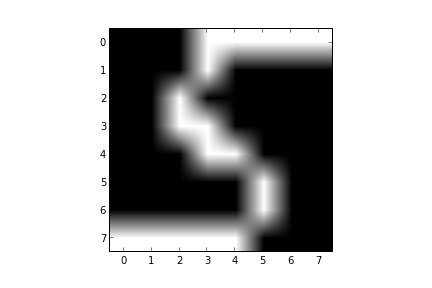
\includegraphics[height=3cm]{boltzmann_01.png}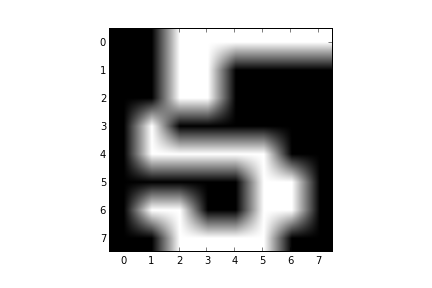
\includegraphics[height=3cm]{boltzmann_02.png}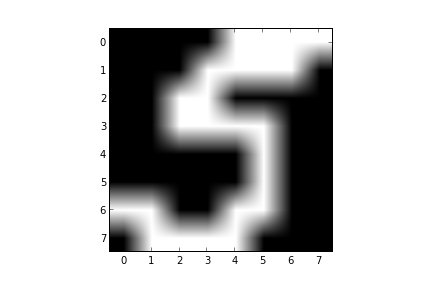
\includegraphics[height=3cm]{boltzmann_03.png}


Bu goruntuleri tanimak icin BM kullanalim. Egitim ve test olarak veriyi
ikiye ayiracagiz, ve egitim seti her etiketin $W$'sini ogrenmek icin
kullanilacak. Daha sonra test setinde her veri noktalarini her uc BM'ye
ayri ayri ``sorup'' o test verisinin o BM'e gore olasiligini alacagiz, ve
hangi BM daha yuksek olasilik donduruyorsa etiket olarak onu kabul
edecegiz. Hangi BM daha yuksek olasilik donduruyorsa, o BM ``bu verinin
benden gelme olasiligi yuksek'' diyor demektir, ve etiket o olmalidir.

\inputminted[fontsize=\footnotesize]{python}{testbm.py}

\begin{minted}[fontsize=\footnotesize]{python}
!python testbm.py
\end{minted}

\begin{verbatim}
Iteration 0
Iteration 10
Iteration 20
Iteration 0
Iteration 10
Iteration 20
Iteration 0
Iteration 10
Iteration 20
Boltzmann Makinasi 0.975
KNN 0.975
\end{verbatim}

Sonuc yuzde 97.5, oldukca yuksek, ve KNN metotu ile ayni sonucu aldik, ki
bu aslinda oldukca temiz / basit bir veri seti icin fena degil.

Biraz Hikaye

Boltzman Makinalariyla ilgilenmemizin ilginc bir hikayesi var. Aslinda bu
metottan haberimiz yoktu, ayrica mevcut isimizde 0/1 iceren ikisel
verilerle cok hasir nesirdik, ve bu tur verilerde ikisel iliskiler
(cooccurence) hesabi iyi sonuclar verir, ki bu hesap basit bir matris
carpimi ile elde edilir.

\begin{minted}[fontsize=\footnotesize]{python}
import numpy as np
A = np.array([\
[0.,1.,1.,0],
[1.,1.,0, 0],
[1.,1.,1.,0],
[0, 1.,1.,1.],
[0, 0, 1.,0]
])
c = A.T.dot(A).astype(float)
print c 
\end{minted}

\begin{verbatim}
[[ 2.  2.  1.  0.]
 [ 2.  4.  3.  1.]
 [ 1.  3.  4.  1.]
 [ 0.  1.  1.  1.]]
\end{verbatim}

Burada bakilirsa 2. satir 3. kolon 3 degerini tasiyor cunku 2. ve
3. degiskenlerin ayni anda 1 olma sayisi tam olarak 3. Sonra acaba bu
bilgiyi veri uzerinde hesaplayip bir kenara koysak bir dagilim gibi
kullanamaz miyiz, sonra yeni veri noktasini bu ``dagilima sorabiliriz''
diye dusunduk. Biraz matris carpim cambazligi sonrasi, yeni veri noktasi
icin

\begin{minted}[fontsize=\footnotesize]{python}
x = np.array([0,1,1,0])
print np.dot(np.dot(x.T,c), x) / 2
\end{minted}

\begin{verbatim}
7.0
\end{verbatim}

gibi sonuclar alabildigimizi gorduk; Bu degerin iliski matrisinin tam
ortasindaki 4,3,3,4 sayilarinin toplaminin yarisi olduguna dikkat
edelim. Yani $x$ carpimi iliski matrisinin sadece kendini ilgilendiren
kismini cekip cikartti, yani 2. ve 3. degisenleri arasindaki iliskiyi
toplayip aldi.

Buradan sonra, ``acaba bu bir dagilim olsa normalizasyon sabiti ne
olurdu?'' sorusuna geldik, ki [4] sorusu buradan cikti ve bu soruya bomba
bir cevap geldi. Sonra diger okumalarimiz sirasinda Boltzmann Dagilimina
ulastik, bu dagilimin ek olarak bir $\exp$ tanimi var (ki turev alimi
sirasinda bu faydali), ve tabii ogrenim icin daha net bir matematigi
var. Biz de maksimum olurluk ile [4]'teki fikrin sayisal kovaryansa
ulastirip ulastirmayacagini merak ediyorduk, BM formunda verisel kovaryans
direk elde ediliyor. Boylece BM konusuna girmis olduk. 

Fakat daha iyi haber BM'in, Kisitli BM (RBM) icin bir ziplama tahtasi
olmasi, zaten RBM'den sonra Derin Ogrenim (Deep Learning) konusu geliyor,
cunku DO birden fazla RBM'lerin ust uste konmus hali. 

[1] Information Theory, Inference and Learning Algorithms, D. MacKay, sf. 523

[2] \url{http://nbviewer.ipython.org/gist/aflaxman/7d946762ee99daf739f1}

[3] \url{http://math.stackexchange.com/questions/1095491/from-pxw-frac1zw-exp-bigl-frac12-xt-w-x-bigr-to-sigmoid/}

[4] \url{http://math.stackexchange.com/questions/1080504/calculating-the-sum-frac12-sum-xt-sigma-x-for-all-x-in-0-1-n}


\end{document}
